The first conclusion of LQG is that GR and QM do not contradict each other. A quantum theory that reduces to GR as its classical limit seems to exist. The work was not small and more is needed to represent the dynamics, but, in the end, a theory was produced which, more than merging GR and QM, it coherently adapts the generally relativistic aspects of GR to a quantization process, which is in general mathematically ill--posed.\, What is fundamental is that LQG follows in many aspects the deductive process that led Einstein himself to his revolutionary geometric theory of gravity, and chooses to best preserve its covariance characteristics and adapt them to a quantum interpretation. Of course, this could not be done by avoiding the choice of some physical postulates---which in this case has been to represent quantum states discretized on lattices---whose truthfulness actually shapes the theory, which can only be proven true by experiments (CFR. \cite{baggot}).\, While LQG may not offer the definitive quantum portrait of spacetime, it undeniably stands as a well--founded proposal for a generally covariant quantum field theory, particularly from a mathematical perspective. The dynamical nature of the spacetime metric field mandates its determination through field equations, eschewing a--priori fixation and safeguarding the foundational tenet of background--independence throughout the quantisation process. %Although it does not turn out to be the true quantum description of spacetime, LQG is certainly a first and working proposal for a generally covariant quantum field theory, at least from a mathematical point of view. Indeed, the spacetime metric field, being a dynamical variable, must be determined a--posteriori by field equations, and cannot be a--priori fixed. 

Technically speaking, we had a gauge--natural field theory in $\mathcal{F}(P)\times_{\M^{1,3}}\Con(P)$, with structure bundle $P\to\M^{1,3}$ being a principal $\SL(2,\C)$--bundle over the spacetime, in the dynamical variables $(e^I,\omega^{IJ})$, so--called Holst theory, being constrained by both the gauge and the diffeomorphism covariance. As a matter of fact, Holst theory, being dynamically equivalent to GR, also imposes topological obstructions on the spacetime, which has to be globally hyperbolic, hence a farther constraint appears, related to the evolution in time of space. Once the constraint equations have been grossed up, such a theory reduces to a $\SU(2)$--gauge--natural theory in the dynamical variables $(e^a,\kappa^i,\A^i)$, the physical states being represented by gauge equivalence classes of $\SU(2)$--connections $[\A]$ on the leaves of a foliation of $\M^{1,3}$, which turn out to be space--like by construction, with respect to the metric induced by the frame $e^a$. At this stage, the quantization procedure is initiated by discretizing the gauge field $\A$, paving the way for the construction of the Hilbert quantum space. Here, kinematical states are defined as $\SU(2)$--functionals $\Psi[\A]$, embodying the foundational principles of quantum mechanics. Imposing the symmetries encoded in the constraint equations, we ensure compliance with the main axioms of quantum mechanics within the confines of a separable Hilbert space of gauge and $\Diffeo_*$ covariant states representing the gravitational field.\, In the end, operators that restrict to the invariant states turn out to correspond to a Lie algebra of geometric observables which stand for the quantisation of the classical geometry of a tetrahedron. The overarching perspective offered by LQG is that the gravitational field, at its core, is depicted through quantum spin networks intricately woven on lattices of $4$--valence nodes, the links being represented by discrete spin connections---almost exactly like the famous picture of Rovelli's books.
\begin{figure}[ht]
    \centering
    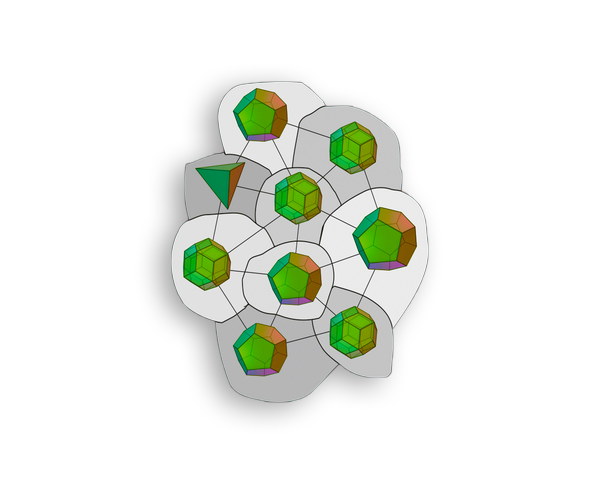
\includegraphics[scale=1.4]{images/spin_networks.png}
    \caption{© Copyright from \emph{L'ordine del tempo} by Carlo Rovelli.}
    %\label{fig:enter-label}
\end{figure}

Within this paradigm, geometric observables undergo quantum fluctuations, shedding light on the intrinsic uncertainty that hence characterizes spacetime at its most fundamental level, as one would expect from a quantum theory of space geometry. 

It is worth highlighting that our current effort has primarily centered on the integration of kinematic constraints derived from gauge and natural symmetries. However, as we progress, it becomes evident that our exploration should extend to include the incorporation of the Hamiltonian constraint, due to the globally hyperbolic structure of spacetime. This additional facet is pivotal as it not only enriches our understanding but also serves as a crucial component in the formulation of spin foams, which are so related to the quantum dynamics of spacetime and should allow to reach an utter viewpoint on the quantum spacetime geometry.\\

We acknowledge that this presentation deviates from historical LQG in several aspects:

\begin{itemize}
\item We embark on a mathematically grounded examination of the main objects of differential geometry that the theory involves, particularly connections and their curvature, shedding light on various aspects crucial for subsequent advancements. This is done along the whole Chapter 1.
\item The BI reduction process, as detailed in Section \ref{BI_red}, is underpinned by a meticulously demonstrated argument grounded in the principles of differential geometry, as discussed in \cite{kobayashi1} and \cite{Orizzonte}: the splitting argument is made on the spacetime, not in space, as it is usually done in the literature. Among its various facets, this argument elucidates a dimensional sensitivity inherent in deriving the Barbero--Immirzi connection. For instance, in four-dimensional spacetimes, such reductions are parameterized by a $\beta\in\R$, distinguishing it as a kinematical quantity distinct from the dynamical Holst parameter $\gamma\in\R\setminus\{0\}$. Moreover, in spacetimes of dimension $3$ or strictly greater than $4$, the parameter turns out to be $\beta=0$, offering intriguing avenues for further mathematical exploration in this direction.
\item In the evolutionary interpretation of Holst theory, the canonical analysis offers a refined approach, yielding boundary equations directly from mathematical principles rather than resorting to ad--hoc definitions. Furthermore, a fresh interpretation of the covariant Cauchy problem emerges with the formalization of Cauchy bubbles and pre--quantum states---see \cite{LN2}.
\item In the implementation of the constraint equations on the quantum space of kinematical states, imposing the gauge and diffeomorphism invariance leads us to invariant states that represent the spatial aspect of the gravitational field. These states are characterized by (possibly knotted) spin networks residing within a separable Hilbert space modeled on lattices. Another noteworthy outcome of our discussion is that, as we delve into the realm of spin knots, the direct relationship with the manifold structure fades away. {Indeed, one can examine what happens to the corresponding functionals when one changes the way links are knotted, resulting in spin knots being insensitive to the knotting of links: they depend only on the abstract lattice. This implies that upon implementing $\Diffeo_*$--invariance, the perceived embedding of the lattice dissipates, leaving behind only abstract lattice structures at the quantum level}.

\item We have introduced operators for holonomies, which are contingent upon the fields $\A^i_a(k)$, as well as momenta operators, which are dependent on the densitized triads $\E^a_i(k)$. Through precise definitions of these operators, the need for postulating commutators is obviated, allowing for straightforward computation within the framework of our model.
  
\end{itemize} 







  
%- Embracing an abstract lattice-only approach (as discussed in LN7), we observe a departure from the traditional emphasis on manifold structure, allowing for a more flexible framework.
  
%- By providing precise definitions for operators governing holonomies and momenta, which depend respectively on connections and densitized triads, we eliminate the need for postulating commutators, thus enabling straightforward computation.

%$$\vdots$$
%Diciamo qui che questa presentazione è diversa da LQG storica: i punti che sono stati approcciati diversamente sono

%\begin{itemize}
   % \item mathematical--founded study of connections wich clarifies many aspects useful in the next steps
    
    %\item BI reduction (C\&P of LN3) the reduction procedure to obtain Barbero-Immirzi connection is dimensional sensitive, as the original Holst dynamics is.

    %\item Canonical analysis in the evolutionary reduction getting boundary equations as mathematically derived, not as a--doc definitions.
    
   % \item Abstract lattice only (C\&P of LN7) "the manifold structure has mainly slipped away"

    %\item We have introduced operators for holonomies, which are contingent upon the connection, although not directly derived from the fields $\A^i_a(k)$, as well as momenta, which are dependent on the densitized triad $\E^a_i(k)$. Through precise definitions of these operators, the need for postulating commutators is obviated, allowing for straightforward computation within the framework of our model.
    
   % We gave operators for holonomies (which depend on the connection, though not directly from the fields $\A^i_a(k)$) and momenta (which depend on the densitized triad $\E^a_i(k)$). Since we defined these operators precisely, we do not need to postulate commutators, we simply can compute them.
%\end{itemize}
As mentioned earlier, we have advanced LQG to the point where we can describe a quantum geometry of spatial leaves of spacetime composed of quantum tetrahedra, whose geometric characteristics are subjected to uncertainty. The next step would be to extend this framework to encompass the entire spacetime, by including consideration of the Hamiltonian constraint. {As a matter of fact, in order to solve the Hamiltonian constraint into our Hilbert quantum space, it is convenient to begin by introducing the area and volume operators. This supports the interpretation of the quantum Hamiltonian operator in terms of their commutators and underscores the fact that geometric observables, such as areas and volumes, are kinematical and remain independent of the Hamiltonian operator, being instead dynamical.}

As a matter of fact, path--quantisation is the prevailing approach that has been pursued, within the LQG community, to reach such a quantum description of spacetime. However, the discussion presented in this thesis suggests that one can see quantisation also in an alternative more algebraic point of view: one could potentially extend the arguments discussed throughout Chapter 3 directly to spacetime, aiming to handle the dynamical physical states of spacetime (so--called spin foams) through a lattice formalism involving the irreducible representations of $\SL(2,\C)$ directly. These representations are infinite--dimensional, given that $\SL(2,\C)$ is a non--compact Lie group. This approach opens up new avenues for exploration within the realm of LQG. %paving the way for a deeper understanding of the quantum nature of spacetime.

Another possible way is to frame the discussion in the context of differential topology. As we have observed throughout our exploration, any relativistic theory, including standard GR, can be viewed as a field theory on a bare manifold. This mathematical setting is well--studied in differential topology and offers a rich framework for theoretical investigations. A proposed approach involves utilizing CW--complexes to delve into the realm of spin foams, such objects living in the natural category of loops' homotopies. Moreover, the \emph{geometric algebra} of Grassmann constitutes a promising and only partially explored framework for setting up the final developments of kinematical LQG discussed in this work, offering a way to making arise the geometry of tetrahedra naturally, instead of recovering and studying it a--posteriori, in the arena of multilinear algebra---see \cite{blake} for Whitehead's book on Grassmann geometric algebra. These alternative perspectives could promise to shed new light on the intricate interplay between geometric structures and quantum phenomena in spacetime.

Despite the four--dimensional nature of our physical spacetime, LQG exhibits a remarkable adaptability to any dimension which is shared by GR. This characteristic prompts an exploration into a $3$--dimensional formulation of LQG, aiming to uncover traits that may shed light on new aspects not readily apparent in the original theory. Moreover, it offers a remarkable laboratory to test ideas of loop quantisation (see Section 9.6 of \cite{pullin2} and Section 9.3.1 of \cite{rov1}). This endeavor should involve delving into the representations of $\Spin(1,2)$ instead, which is infinite dimensional, being isomorphic to $\SL(2,\R)$---as well as $\SL(2,\C)$, whose irreducible representations aim to describe spin foams---along with its $\Spin(2)\cong\mathrm{U}(1)$--reduction, allowing finite--dimensional irreducible representations, being $\mathrm{U}(1)\cong\mathbb{S}^1$ compact, alike to the approach taken for $\mathrm{Spin}(1,3)$ and $\mathrm{Spin}(3)$, along the whole Chapter 2.\\

Concluding, the discussion on the gravitational field revealed a natural quantisation of space geometry that can be studied independently. Here, I followed an original approach by studying the algebra of invariant operators rather than defining individual cases of invariant operators, as in the literature. This approach proved to be interesting because one could use the standard tools built for analyzing algebra representations. For example, one can detect the maximal commuting sub--algebras of the observables' algebra, providing quantum numbers' choices and allowing to compute the quantum behavior of the remaining quantities.

From this perspective, LQG reduces to the choice---at each node---of areas and volumes as compatible quantities, having spin networks as eigenstates, enabling the definition of other invariant operators (such as the other dihedrals) that encompass the quantum aspects of the considered geometry.


%Cosa si può sperare di fare dopo:

%\begin{itemize}
 %   \item C\&P of LN9 per nuova approccio a spinfoams rifacendo tutto con le rappresentazioni infinito dimensionali di $\SL(2,\C)$
  %  \item As we noticed along the way, mathematically speaking, any relativistic theory (and standard GR) is a field theory on a bare manifold, a setting which in mathematics is called differential topology; proposta di approccio a spinfoams con CW--complexes

   % \item Even if the spacetime of our physical world is $4$--dimensional, the theory does adapt to any dimension. It is for this reason that, in conclusion, I will discuss an attempt of a $3$--dimensional formulation of LQG, looking for some traits that can shed light on new aspects that may not be manifest in the original theory.
   % $$\vdots$$
    %Questo involverebe le rappresentazioni (infinito dimensionali) di $\SL(2,\R)$ e le sue $\U(1)$--reduction ($\U(1)\cong\S^1$ compatto, simile a quanto fatto per $\Spin(1,3)$ e $\Spin(3)$)
%\end{itemize}